
\chapter{Stammdatenpflege}
\label{chap:data}

\section{Stammdatenpflege}

\subsection{Planungsabschnitte (Perioden)}

Planungsabschnitte werden mit der Ressource \texttt{Perioden} in Untis modelliert. Diese Ressourcen sind bereits eingepflegt. Man kann zwischen den jeweiligen Perioden mittels eine Auswahlbox in der obere Menüleiste zwischen den jeweiligen Perioden wechseln. Die Semester sind in der Regel der Hauptplanungsabschnitt an der THM, das Schuljahr hingegen ist für die Pflege von Stammdaten gedacht.\\

\begin{wrapfigure}{r}{0.25\textwidth}
	\vspace{-14pt}
	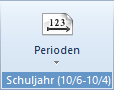
\includegraphics[width=.24\textwidth,right]{perioden}
	\vspace{-15pt}
	\caption{Perioden}
	\label{fig:mf-sg}
\end{wrapfigure}

\noindent
\textbf{Die Pflege der Stammdaten von Gruppen, Räume und Dozenten muss in der Periode ``Schuljahr" gemacht werden.} Wenn Daten in der Schuljahr-Periode eingepflegt sind, werden die neuen Daten, bzw. Änderungen, automatisch im Winter- und Sommersemester Perioden ersichtlich. Sollten neue Stammdaten oder Änderungen an bestehenden in die Winter- oder Sommersemester Perioden eingepflegt werden, sind diese Daten nur in diese eine Periode ersichtlich. Das führt zwangsläufig zu Dateninkonsistenzen.

\subsection{Name und Langname}

Bei einzelne Datensätze ist \texttt{Name} ein eindeutiger Schlüsselwert, der z.B. das schnelle eintippen dieser Ressource in Untis ermöglicht. Er soll dementsprechend so kurz und aussagekräftig wie möglich, gehalten werden. Der \texttt{Langname}, bzw. \texttt{Nachname}, hingegen enthält den tatsächlichen Namen der jeweilige Ressource. \textbf{Bei einzelne Datensätze sind Name und Langname immer Pflicht}.

\newpage

\subsection{Externer Name}
\label{sec:ext-name}

\texttt{Ext. Name} ist ein fachbereichsübergreifender Schlüsselwert. Er ermöglicht die Sicht auf die Planung der Ressource außerhalb des eigenen Fachbereiches. Für Räume ist diese Angabe Pflicht. Gruppen und Dozenten, die für fachbereichsübergreifende Planungen eingesetzt werden (wie z.B. im Studiengang Bioinformatik, SuK Veranstaltungen bei ME, oder Dozenten aus den Dienstleistungsfachbereichen) sollten ebenfalls einen solchen externer Name haben. Sollte eine benötigte Ressource noch nicht in den Stammdaten eines Fachbereiches eingetragen sein, so schicken Sie mir bitte ein Email - ich werde die diese Ressource dann zentral einpflegen und freigeben.

\section{Spezielle Ressourcen}

Spezielle Ressourcen sind solche, die nur als Attribute für andere Ressourcen verwendet werden: Studiengänge und Beschreibungen. Die Stammdatenpflege dieser Ressourcen erreicht man am leichtesten, indem man \texttt{Dateneingabe} in der Reiterleiste auswählt, \texttt{Sonstige Daten} aufklappt und \texttt{Studiengänge} oder \texttt{Beschreibungen} auswählt.\\

\begin{figure}[h]
	\centering
	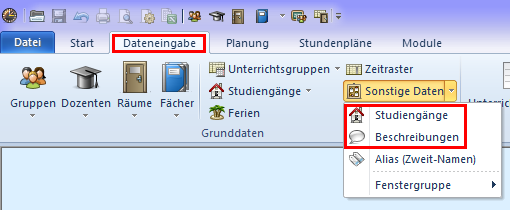
\includegraphics[width=.8\textwidth]{spezielle-daten-menu}
	\vspace{-5pt}
	\caption{Menüführung: spezielle Daten}
	\label{fig:spezielle-daten-menu}
\end{figure}

\subsection{Studiengänge (Abteilungen)}

Studiengänge werden an der THM Gruppen zugeordnet. Die damit implizierte Aussage ist: Gruppen gehören Studiengänge. Man könnte auch Dozenten, Räume und Fächer Studiengänge zuordnen. Dies würde wegen unserer weiteren Modellierung keine weitere Auswirkung haben und ist daher nicht nötig.\\
\\
THM Organizer verwendet Studiengänge um die Navigation für Gruppenpläne zu gestalten.\\

\newpage

\begin{wrapfigure}{r}{0.4\textwidth}
	\centering
	\vspace{-4pt}
	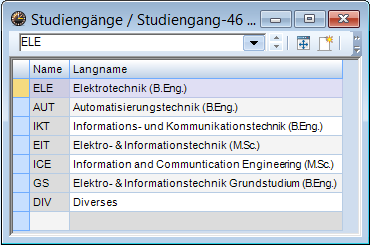
\includegraphics[width=.38\textwidth]{studiengange}
	\vspace{-5pt}
	\caption{Studiengänge}
	\label{fig:studiengange}
\end{wrapfigure}

\noindent
\texttt{Name}: Der Name besteht aus wenigen aber aussagekräftigen Buchstaben. Existiert der Studiengang als Bachelor und Master-Studiengang, so werden diese, getrennt durch einen Punkt, mit ``B" \hspace{1pt} bzw. ``M" \hspace{1pt} erweitert (Bsp.: Informatik Bachelor bzw. Master:  I.B bzw. I.M).\\

\noindent
\texttt{Langname}: Der Name des Studiengangs mit offizieller Abkürzung des Abschlusses in runden Klammern dahinter. Dieser Wert wird öffentlich verwendet in die Darstellungen von Untis und THM Organizer.

\subsection{Beschreibungen}

An der THM wird diese Ressource verwendet, um Fachkompetenzen, Raumkategorien und Unterrichtsmethoden zu modellieren. In Untis gibt es teilweise ähnliche Angaben, sie lassen sich aber nicht einstellen und sind deshalb für unsere Zwecke nicht verwendbar.\\
\\
Sollte diese Angabe bei der Dozent, Raum oder Fach fehlen wird der Plan nicht in der Navigation in Organizer erscheinen.\\

\noindent
{\large Attribute\par}
\vspace{8pt}

\begin{wrapfigure}{r}{0.4\textwidth}
	\centering
	\vspace{-14pt}
	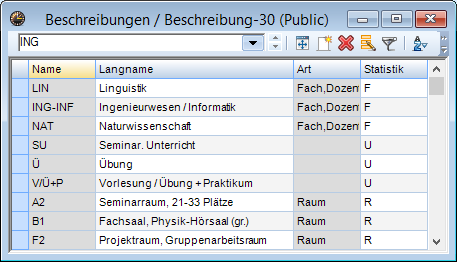
\includegraphics[width=.38\textwidth,right]{beschreibungen}
	\vspace{-15pt}
	\caption{Beschreibungen}
	\label{fig:beschreibungen}
	\vspace{-35pt}
\end{wrapfigure}

\noindent
\texttt{Art}: Diese Angabe ist für uns unbrauchbar und lässt sich leider nicht ausblenden. Daher bitte ignorieren.\\

\noindent
\texttt{Statistik}: Diese Angabe ist Pflicht und wird verwendet, um die Verwendung der Ressource festzulegen.\\

\vspace{9pt}

\subsubsection{Fachkompetenzen}
\label{subsec:fachkompetenzen}

Die Angabe zu den Fachkompetenzen gibt eine grobe Zuordnung der Ressourcen zu bestimmten fachlichen Bereichen vor.\\
\\
Derzeit sind die Namen und Langnamen nach einem von Herr Kneisel entworfenes System aufgebaut. Demnach besteht ein Fachkompetenz aus Basis-Kompetenzen, die jeweils durch drei Buchstaben gekennzeichnet sind. Diese entsprechen einem recht groben Themengebiet wie Naturwissenschaft oder Bauingenieurwesen. Zusätzlich gibt es die Möglichkeit, kombinierte Kompetenzen zu verwenden. Deren Namen setzen sich aus den Bezeichnern von zwei Basis-Kompetenzen, verbunden durch einen Bindestrich zusammen. Ihr Langname ergibt sich durch die Langnamen der Basis-Komponenten, getrennt durch einen Schrägstrich ``/". Fachkompetenzen sind in der Spalte \texttt{Statistik} durch den Buchstaben ``F" \hspace{1pt} gekennzeichnet.\\

\begin{quote}
	\textit{Hier wäre eine Überarbeitung des Systems grundsätzlich wünschenswert. Beispielsweise hat Fachbereich Wirtschaft, zusätzlich zu den Einträgen vom Kneisel'sche System, neun Schwerpunkte, wie Mittelstand oder Marketing. Diese sind um einiges aussagekräftiger und relevanter sowohl für Studenten als auch für Dozenten.}
\end{quote}

\noindent
THM Organizer verwendet diese Angaben für die Stundenplan-Navigation für Dozenten und Fächer, sowie die für die Gruppierung von Fächer im Modulhandbuch.

\subsubsection{Raumkategorien}
\label{subsec:room-category}

Der Name und der Langname beziehen sich auf einem System, entwickelt von Herr Deniffel für die THM, wonach die Namen den Raumtyp und Aussagen über dessen Kapazität oder Ausstattung kodieren.\\
\\
Der Name besteht meist aus einer Buchstabe und einer Zahl. ``A" steht beispielsweise für einen  Seminarraum oder Hörsaal, wohingegen ``D" ein Rechnerraum kennzeichnet. Die Zahlen beziehen sich auf Raumeigenschaften wie Größe oder Ausstattung. Bei A2 heißt das ``2" 21 bis 33 Sitzplätze, bei D2 hingegen heißt die ``2", dass sich in dem Raum eine fachspezifische Ausstattung befindet. Der Langname ist eine von Kommata getrennte Auflösung dieser zwei Teile. Bei Raumkategorien wird ein ``R" in der Statistik Spalte eingetragen.\\
\\
Eine vollständige Liste der Raumkategorien befindet sich im \secref{sec:dennifel}.\\
\\
THM Organizer verwendet diese Angaben für die Stundenplan-Navigation für Räume.\\

\subsubsection{Unterrichtsmethoden}

Unterrichtsmethoden beschreiben die Lehrform eines Unterrichts.\\

\begin{wrapfigure}{r}{0.35\textwidth}
	\vspace{-14pt}
	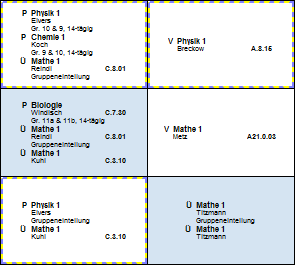
\includegraphics[width=.34\textwidth]{MethodsUntis}
	\vspace{-5pt}
	\caption{Mögliche Darstellung von Unterrichtsmethoden in Untis}
	\label{fig:methoden-untis}
	\vspace{-5pt}
\end{wrapfigure}

\noindent
Der Name besteht meist aus einem, manchmal auch zwei, Buchstaben, wie ``V" für Volesung, "L" für Labor oder "SU" für Seminaristischen Unterricht, der Langname entsprechend der ausführliche Schreibweise. Sollte ein Unterricht mehrere Methoden verwenden, können auch hier Hybride-Methoden verwendet werden, indem man die einfachen Angaben durch ein ``/" trennt. Beispielsweise ``V/Ü"  für Vorlesung oder Übung, oder ``S/P" für Seminar oder Praktikum. Für Unterrichtsmethoden ist die entsprechende Statistik Angabe ``U".\\
\\
In Untis können diese Angaben so eingerichtet werden, dass sie auch mit ausgegeben werden. Eine mögliche Darstellung finden Sie in \figref{fig:methoden-untis}. In THM Organizer wird diese Angabe als Teil des Unterrichtsnamen immer ausgegeben.\\

\section{Gruppen}

\begin{wrapfigure}{r}{0.08\textwidth}
	\vspace{-70pt}
	
\includegraphics[width=.08\textwidth]{gruppen-menu}
\end{wrapfigure}

\vspace{25pt}

Gruppen, auch Klassen in Untis genannt, dienen zur Strukturierung von Studiengängen. Diese sind oft nach Semestern strukturiert (z.B. "1.Semester"), manchmal nach Schwerpunkt ("Praktische Informatik"), manchmal auch nach Kombinationen von Semestern und Schwerpunkten ("Schwerpunkt Marketing im 4.Semester"). Gruppen fassen immer eine Menge von Unterrichten zusammen, die von einer Gruppe von Studierenden besucht werden.\\
\\
Die Stammdatenpflege der Gruppen erreicht man, indem man in der Reiterleiste \texttt{Start} aktiviert hat, \texttt{Gruppen} aufklappt und \texttt{Stammdaten} auswählt. Wie bei allen Dozenten und Räumen, sollten Sie sicherstellen, dass ihre \texttt{Periode} auf ``Schuljahr" \hspace{1pt} steht.

\begin{figure}[h]
	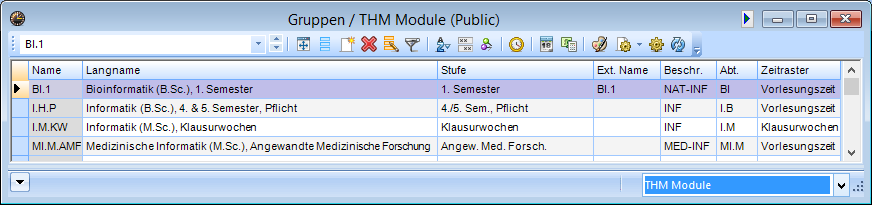
\includegraphics[width=1\textwidth]{Gruppen}
	\vspace{-15pt}
	\caption{Gruppen}
	\label{fig:groups}
\end{figure}

\noindent
{\large Attribute\par}
\vspace{8pt}

\noindent
\texttt{Name}: Beinhaltet Hinweise auf den jeweiligen Studiengang, sowie deren spezifische Untergliederung. Typischerweise mit Punkten getrennt.\\

\noindent
\texttt{Langame}: Der ausgeschriebene Name des Studiengangs mit Abschluss in runden Klammern, gefolgt von Untergliederungsteile, getrennt durch Kommas.\\

\noindent
\texttt{Ext. Name}: (Pflicht bei Fachbereichsübergreifende Gruppen, sonst optional, siehe auch 
\secref{sec:ext-name})\\

\noindent
\texttt{Stufe}: Eine Kurzfassung der Untergliederung. Diese Angabe wird als Name in der Stundenplan-Navigation in THM Organizer benutzt.(Pflicht)\\

\noindent
\texttt{Beschr.} (Fachkompetenz): Assoziiert die Gruppe mit einer Fachkompetenz. (Pflicht. Siehe \secref{subsec:fachkompetenzen}))\\

\noindent
\texttt{Abt.} (Studiengang): Assoziiert die Gruppe und ihre Unterrichte mit einem Studiengang. (Pflicht)\\

\newpage

\noindent
\texttt{Zeitraster}: Assoziiert die Gruppe mit einem Zeitraster. Standardmäßig ist der Wert dieser Spalte ``Hauptzeitraster". Falls Multi-Zeitraster verwendet wird, kann man eingepflegte Zeitraster auswählen. (Pflicht. Wird automatisch mit einem default Wert gefüllt. Siehe auch \nameref{sec:zeitraster})

\subsubsection{Zeitraster \& Klausurwochen}
\label{sec:zeitraster}

Zeitraster legen die Blöcke fest in dem man Unterrichtsinstanzen unterbringen kann. An der THM haben wir bisher zwei feste Zeitraster, eine für Vorlesungen und eine für die Klausurwochen. Solche Zeitraster sind in Untis mit Gruppen assoziiert. Das hat Konsequenzen für unsere Modellierung der Klausurwochen, denn wenn Zeitraster nur mit Gruppen assoziiert werden können, muss es sinnvolle Gruppen geben, um die Klausuren der Klausurwochen zu modellieren.\\
\\
In Fachbereich MNI haben wir eine Klausurwochen-Gruppe pro Studiengang angelegt. Diese verwenden die zweistündige Zeitraster der Klausurwochen. Klausuren können damit Untis-intern recht gut abgebildet werden. Zur Zeit kann Untis die zusätzliche Raster aber nicht exportieren, dass hat als Folge, dass Organizer sie deshalb noch nicht korrekt anzeigen kann.\\

\section{Dozenten}

\begin{wrapfigure}{r}{0.08\textwidth}
	\vspace{-70pt}
	
\includegraphics[width=.08\textwidth]{dozenten-menu}
\end{wrapfigure}

\vspace{25pt}

Dozenten, auch Lehrer in Untis genannt, bezeichnen festangestellte Dozenten, Lehrbeauftragte, Tutoren, Vortragende, Seminarleiter. Kurz gesagt, alle die für eine Veranstaltung oder einen Unterricht verantwortlich sind.\\
\\
Sie erreicht man von der \texttt{Start} Leiste in dem man \texttt{Dozenten} aufklappt und \texttt{Stammdaten} auswählt.\\

\begin{figure}[h]
	\centering
	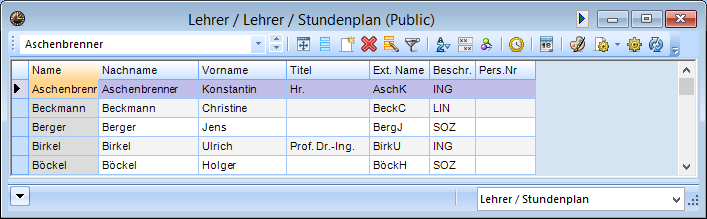
\includegraphics[width=.8\textwidth]{Teachers}
	\vspace{-5pt}
	\caption{Dozenten}
	\label{fig:teachers}
\end{figure}

\noindent
{\large Attribute\par}
\vspace{8pt}

\noindent
\texttt{Name}: Typischerweise wird hier den Nachnamen eingetragen, bei Uneindeutigkeiten können Buchstaben aus den Vornamen und ggf. weitere Nachnamen hinzugefügt.\\

\noindent
\texttt{Nachname}: Die Nachnamen des Dozenten.\\

\noindent
\texttt{Vorname}: Die Vornamen des Dozenten.(Empfohlen)\\

\noindent
\texttt{Ext.Name}: (Pflicht bei Dozenten die in mehreren Fachbereiche tätig sind, sonst Optional, siehe auch 
\secref{sec:ext-name})\\

\noindent
\texttt{Beschr.} (Kompetenz): Assoziiert der Dozent mit einer Fachkompetenz. (Pflicht, siehe   \secref{subsec:fachkompetenzen}))\\

\noindent
\texttt{Pers.Nr} (THM Benutzerkennung): Die THM Benutzerkennung des Dozenten. Erlaubt die eindeutige Zuordnung des Dozenten und ermöglicht ggf. die Verlinkung auf einem Benutzer-Profile aus THM Organizer. (Optional)\\

\section{Räume}

\begin{wrapfigure}{r}{0.08\textwidth}
	\vspace{-80pt}
	
\includegraphics[width=.08\textwidth]{raume-menu}
\end{wrapfigure}

\vspace{35pt}

Räume bezeichnen sämtliche Orte, an denen Unterrichte, Vorträge, Sitzungen und sonstige planungsrelevante Ereignisse stattfinden. Obwohl klassische Veranstaltungsräume, wie Hör- und Seminarräume den Großteil des Raumbestands ausmachen, müssen hier auch außergewöhnliche Örtlichkeiten wie "Grillplatz", "Kongresshalle" oder "Online" aufgeführt sein, damit möglichst ausnahmslos alle Unterrichte mit einem Ort versehen werden können.\\
\\
Von der \texttt{Start} Leiste drückt man klappt man \texttt{Räume} auf und wählt \texttt{Stammdaten} aus.

\begin{figure}[h]
	\centering
	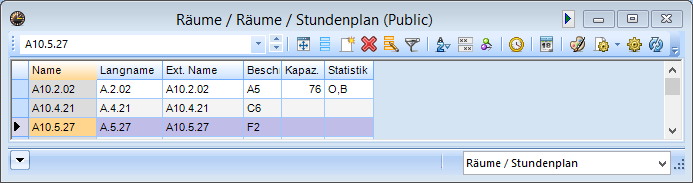
\includegraphics[width=.8\textwidth]{Rooms}
	\vspace{-5pt}
	\caption{Räume}
	\label{fig:rooms}
\end{figure}

\noindent
{\large Attribute\par}
\vspace{8pt}

\noindent
\texttt{Name}: Der Raum Name. Damit die Namen Campus-übergreifend eindeutig sind, wird der Bezeichner für A und C Gebäuden zu ``A10", bzw. ``C10".\\

\noindent
\texttt{Langname}: Die aktuelle Bezeichnung für den Raum.\\

\noindent
\texttt{Ext.Name}: Identisch mit \texttt{Name}. (Pflicht)\\

\noindent
\texttt{Beschr.} (Raumkategorie): Die Kategorie des Raumes. Wird in THM Organizer für Raumplan-Navigation verwendet. (Pflicht, siehe \secref{subsec:room-category})\\

\noindent
\texttt{Kapaz.} (Kapazität): Die Anzahl der Sitzplätze / Rechnerplätze. (Optional)\\

\noindent
\texttt{Statistik} (Ausstattung): Einstellige Bezeichner für die Raumausstattung, wie Overhead (O) oder Beamer (B). Die Bezeichner werden durch Kommata getrennt. Diese werden von Untis eingefügt, der Benutzer braucht nur die Buchstaben einzutragen. (\textbf{Optional})\\

\subsubsection{Raumgruppen}

Raumgruppen sind Gruppierungen von Räumen nach z.B. Typ, Ausstattung, Kapazität, Verwendungszweck, oder eine Kombination daraus. In \figref{fig:roomgroups} sieht man drei der Gruppen der Fachbereich MNI verwendet. Die erst Gruppe, LPC, beinhaltet eine Auflistung der Rechnerlabore in Gebäude A20, jeweils von gleichen Typ, mit einer ähnlichen Ausstattung und Kapazität.\\
\\
Die Verwendung von Raumgruppen ist für die Planung nicht zwingend notwendig, sie eine Planung, die unabhängig von konkreten Räumen ist und nur Raumtypen betrachtet. Das ist in den meisten Fällen genau das was man in der Planung möchte, denn häufig ist der konkret Raum nicht wichtig. Mehr dazu in \chapref{chap:lessons}.\\
\\ 
Von der \texttt{Start} Leiste drückt man klappt man \texttt{Räume} auf und wählt \texttt{Raumgruppen} aus.

\begin{figure}[h]
	\centering
	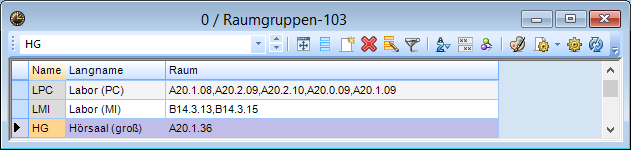
\includegraphics[width=.8\textwidth]{RoomGroups}
	\vspace{-5pt}
	\caption{Raumgruppen}
	\label{fig:roomgroups}
\end{figure}

\noindent
{\large Attribute\par}
\vspace{8pt}

\noindent
\texttt{Raum}: Eine Komma-getrennte Liste der Räume, die dieser Gruppe gehören. (Pflicht, sofern verwendet)\\

\newpage

\section{Fächer}

\begin{wrapfigure}{r}{0.08\textwidth}
	\vspace{-80pt}
	
\includegraphics[width=.08\textwidth]{facher-menu}
\end{wrapfigure}

\vspace{35pt}

Fächer sind die Namensträger für Unterrichte und Unterrichtsinstanzen. Sie geben einen Hinweis darauf, welche Lerninhalte in einem Unterricht oder Unterrichtsinstanz vermittelt werden und sind an der THM (praktisch immer) identisch mit Modulen.\\
\\
Zum Beispiel besteht das Modul ``International Marketing" \hspace{1pt} im Studiengang Unternehmensführung aus mehrere Fächer, im Stundenplan ist nur ein Name für alle solche Fächer gewollt. Im Gegensatz dazu stehen Module wie ``Theorie des Entwerfens I" \hspace{1pt} aus dem Studiengang Bauingenieurwesen, hier sind die Namen der untergeordneten Fächer Einführung ins Entwerfen und Baugeschichte der Ausgabe gewollt und müssen deshalb getrennt eingepflegt werden.\\
\\ 
Fächer haben die besondere Eigenschaft, dass sie nicht in der Periode "Schuljahr" gepflegt werden brauchen, denn jegliche Änderungen an einem Fach sind sofort in allen Perioden sichtbar.\\
\\
Um ein Fach zu erstellen oder zu bearbeiten, muss man in der \texttt{Start} Leiste \texttt{Fächer} aufklappen und \texttt{Stammdaten} auswählen.

\begin{figure}[h]
	\centering
	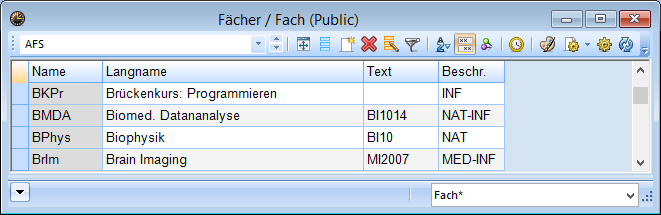
\includegraphics[width=.8\textwidth]{Subjects}
	\vspace{-5pt}
	\caption{Fächer}
	\label{fig:subjects}
\end{figure}

\noindent
{\large Attribute\par}
\vspace{8pt}

\noindent
\texttt{Text} (Modulnummer): Die Modulnummer des Faches/Moduls. Hier ist entscheidend, wie die Module in LSF abgelegt werden, denn diese Angabe ist notwendig für die automatische Weiterleitung auf Modulbeschreibungen im THM Organizer. Bei Module, die aus mehreren Fächern bestehen, ist es nicht geregelt auf welche Hierarchie-Ebene die Zuordnung zu einer Modulbeschreibung liegt (Modul/Fach). In diesen Fällen sollten wir mit der LSF Verantwörtlichen reden um Klarheit zu beschaffen. (Empfohlen)\\

\noindent
\texttt{Beschr.} (Kompetenz): Assoziiert das Fach mit einer Kompetenz. (Pflicht, siehe \secref{subsec:fachkompetenzen})\\

\section{Verläufe (Unterrichtsgruppen)}
\label{sec:unterrichtsgruppen}

\noindent
Unterrichtsgruppen sind terminliche Begrenzungen von Unterrichten. Dort kann man feste Start- und Enddaten angeben, sowie den Verlauf zwischen diese zwei Daten.\\

\begin{wrapfigure}{r}{0.4\textwidth}
	\vspace{-14pt}
	\centering
	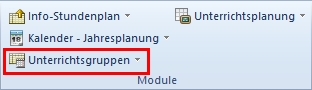
\includegraphics[width=.39\textwidth]{unterrichtsgruppen-symbol}
	\vspace{-5pt}
	\caption{Unterrichtsgruppen im Menü}
\end{wrapfigure}

\noindent
Unterrichtsgruppen findet man in der \texttt{Start} Leiste im Rubrik \texttt{Module}. Es sind bereits in jede Schule Unterrichtsgruppen eingetragen und konfiguriert, diese müssen lediglich den Gegebenheiten der jeweiligen Fachbereiche angepasst werden. Welche Verläufe Ihnen eingerichtet sind und wie deren Lauf gestaltet wird, schlagen Sie am besten im Programm nach.\\

\begin{wrapfigure}{r}{0.4\textwidth}
	\label{fig:unterrichtsgruppen-symbol}
	\centering
	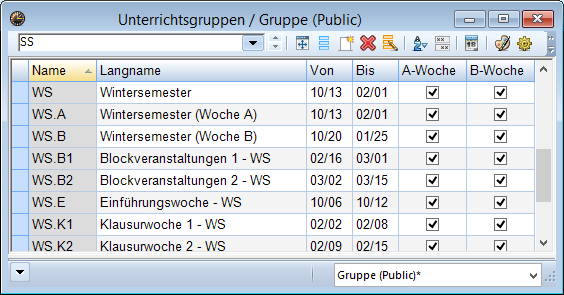
\includegraphics[width=.39\textwidth]{unterrichtsgruppen-ansicht}
	\vspace{-5pt}
	\caption{Unterrichtsgruppen Ansicht}
	\label{fig:unterrichtsgruppen-ansicht}
	\vspace{-115pt}
\end{wrapfigure}

\noindent
{\large Attribute\par}
\vspace{8pt}

\noindent
\texttt{Von}: Das Startdatum der Unterrichtsgruppe. (Pflicht)\\

\noindent
\texttt{Bis}: Das Enddatum der Unterrichtsgruppe. (Pflicht)\\

\vspace{54pt}

\noindent
{\large Kalender\par}
\vspace{8pt}

\begin{wrapfigure}{r}{0.4\textwidth}
	\vspace{-14pt}
	\centering
	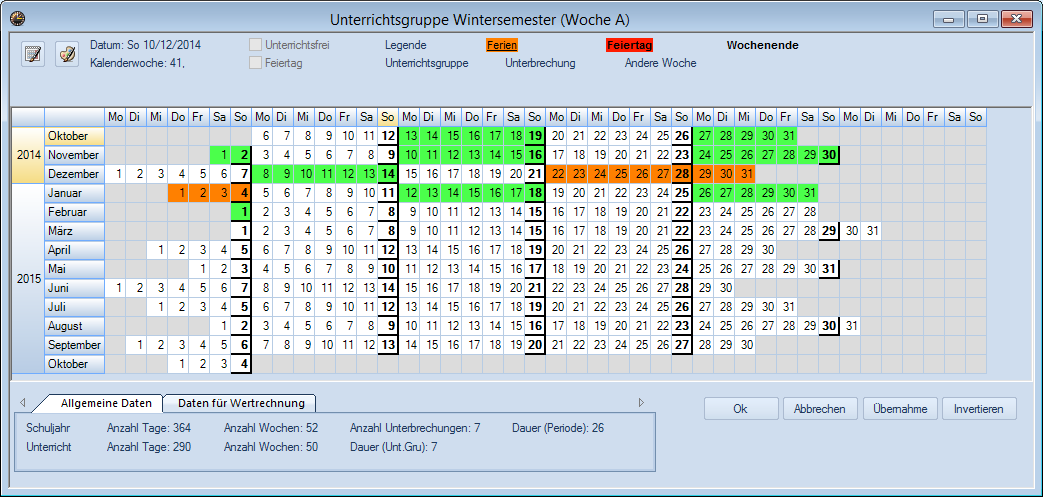
\includegraphics[width=.39\textwidth]{unterrichtsgruppen-kalender-ansicht}
	\vspace{-5pt}
	\caption{Unterrichtsgruppen Kalender}
	\label{fig:unterrichtsgruppen-kalender-ansicht}
	\vspace{14pt}
\end{wrapfigure}

\noindent
Unterrichtsgruppen eignen sich sehr gut dafür die Periodizität von Unterrichten sehr fein auf die Wochen abzustimmen - damit können z.B. vorlesungsfreie Zwischenzeiten (wie Weihnachten) berücksichtigt werden. Hierfür verwendet man die Schuljahres-Ansicht. In dieser Ansicht kann man Datenbereiche überstreichen oder einzelne Tage anklicken, um diese in den Verlauf der Unterrichtgruppe zu übernehmen oder zu entfernen. An grünen Tagen werden assoziierte Unterrichte stattfinden können. An weißen Tagen, sowie orangen (Ferien), werden assoziierte Unterrichte nicht stattfinden können. Schließlich klickt man auf \texttt{Ok} oder \texttt{Übernahme}, um die Änderungen geltend zu machen.\\





